% =========================================================================
% SciPost LaTeX template
% Version 1e (2017-10-31)
%
% Submissions to SciPost Journals should make use of this template.
%
% INSTRUCTIONS: simply look for the `TODO:' tokens and adapt your file.
%
% - please enable line numbers (package: lineno)
% - you should run LaTeX twice in order for the line numbers to appear
% =========================================================================


% TODO: uncomment ONE of the class declarations below
% If you are submitting a paper to SciPost Physics: uncomment next line
\documentclass[submission, Phys]{SciPost}
% If you are submitting a paper to SciPost Physics Lecture Notes: uncomment next line
%\documentclass[submission, LectureNotes]{SciPost}
% If you are submitting a paper to SciPost Physics Proceedings: uncomment next line
%\documentclass[submission, Proceedings]{SciPost}

\usepackage{braket}
\usepackage[ruled, vlined]{algorithm2e}
\usepackage{amsmath, bm}
\usepackage{dsfont}
\usepackage{pythonhighlight}
\SetKwComment{Comment}{$\triangleright$\ }{}

\begin{document}

\begin{center}{\Large \textbf{
			QuCumber: wavefunction reconstruction with neural networks
		}}\end{center}

\begin{center}
	Matthew J.~S.~Beach,
	Isaac De Vlugt,
	Anna Golubeva,
	Patrick Huembeli$^\dag$,
	Roger G.~Melko\textsuperscript{*},
	Ejaaz Merali,
	Giacomo Torlai,
\end{center}

\begin{center}
	%{\bf 1} 
	Department of Physics and Astronomy, University of Waterloo,
	\\Ontario N2L 3G, Canada
	\\
	Perimeter Institute for Theoretical Physics, Waterloo,
	\\Ontario N2L 2Y5, Canada
	\\
	ICFO-Institut de Ciencies Fotoniques, Barcelona Institute of Science and Technology,
	\\08860 Castelldefels (Barcelona), Spain$^\dag$ \\
	* rgmelko@uwaterloo.ca \\
\end{center}

\begin{center}
	\today
\end{center}

% For convenience during refereeing: line numbers
%\linenumbers

\section*{Abstract}
{\bf
	In this post we present QuCumber, an open-source Python package which uses Restricted Boltzmann Machines for the reconstruction of quantum states from measurement data. 
    The use of modern machine learning techniques makes it possible to efficiently learn quantum states and access traditionally challenging many-body quantities which are not directly accessible to experiments. 
    We give examples of how to use QuCumber on positive-real and complex wavefunctions and how to extract meaningful observables such as energy, magnetization and fidelity.
}

\vspace{10pt}
\noindent\rule{\textwidth}{1pt}
\tableofcontents\thispagestyle{fancy}
\noindent\rule{\textwidth}{1pt}
\vspace{10pt}

\section{Introduction}

Scientific progress in controlled quantum systems has allowed for increasingly large-scale devices which can accurately prepare pure quantum states.
As the size of these devices grows to hundreds of qubits, we face the challenge of analyzing highly complex many-body states with a finite set of experimental measurements.
Since the computational power required scales exponentially with the number of qubits, there is a growing interest in using machine learning techniques which can successfully distill meaningful statistics from very large amounts of data.
In this post, we present a software package that can be used to characterize and analyze pure states produced from near-term 
quantum devices by {\it reconstructing} a quantum wavefunction with machine learning methods.

QuCumber is based on Restricted Boltzmann Machines (RBM), an unsupervised generative modelling technique 
used widely in applications~\cite{Smolensky}.
RBMs can represent many complicated objects including handwritten digits, natural images, and many-body wavefunctions~\cite{Torlai2016thermo, CarleoTroyer2017Science, ChenWang2018, GlasserCirac2018}.
An RBM can be interpreted as an approximate graphical representation of a probability distribution. This distribution is defined by the energy of a classical Ising model, with tunable couplings which can be optimized during a training procedure.
With slight modifications, one can represent complex wavefunctions with an amplitude and phase or mixed states~\cite{torlai2018tomography, TorlaiPure} 

The need for QuCumber arises from the growing availability of high quality data obtained from controlled quantum
systems and devices.
QuCumber provides a freely accessible open-source software package that supports wavefunction reconstruction directly from experimental data representing measurements of qubit eigenvalues, spin states, or orbital occupation numbers.
QuCumber is used to optimize the parameters of an RBM to model the most likely quantum state given a series of measurements,
a procedure analogous to the maximum likelihood technique, Bayesian inference or quantum state tomography. 
%however, our method does not scale exponentially with system size.
Once trained, the RBM parameters encode a compressed version of the underlying wavefunction.
New quantum state measurements can then be generated by the RBM, and observables that are otherwise not easily accessible from the original data can be calculated. 
%Examples of which include off-diagonal correlation functions and entanglement entropies~\cite{Torlai2016thermo, torlai2018tomography}. \textcolor{red}{this is not really a sentence...}
%QuCumber builds on previous studies which reconstructed wavefunctions from simulation and experimental data. 
Trained RBMs can be sampled to produce non-trivial measurements such as off-diagonal correlation functions and entanglement entropies~\cite{Torlai2016thermo, torlai2018tomography}.

In this paper, we describe how QuCumber can be used for these and other tasks in characterizing quantum many-body phenomenon on hundreds or thousands of qubits.
In the following, we provide code snippets written in Python 3, using PyTorch with CPU and GPU support~\cite{paszke2017automatic}.
We refer the reader to the full code documentation (\url{https://piquil.github.io/QuCumber/}) for further information on the code structure and operation.


% \subsection{State Reconstruction with RBMs}

% QuCumber allows to reconstruct the approximate wavefunction
% $\psi( \boldsymbol{\sigma} ) = \langle \boldsymbol{\sigma} | \psi \rangle$
% in some fixed basis
% $\{ \vert \boldsymbol{ \sigma} \rangle \}$
% from a set of experimental measurements.
% For instance, the data set could consist of a series of single qubit measurements
% $\vert {\boldsymbol{\sigma}} \rangle = \vert { \sigma}_1~{ \sigma}_2 \dots \rangle$
% in the computational basis obtained by preparing the state and measuring it several times.

% Any set of measurements on a quantum wavefunction is distributed according to the probability distribution defined by Born's rule:
% $p(\boldsymbol{\sigma}) = | \psi( \boldsymbol{\sigma} ) |^2$.
% The goal of QuCumber is to learn the best possible approximation to a wavefunction which underlies a set of measurement data.
% After the parameters of the RBM have been adjusted based on the data set, it becomes a compressed reconstruction of the original target wavefunction.
% New quantum states can now be generated by the RBM, and new observables measured.
% QuCumber implements a simple framework for sampling the reconstructed wavefuntion
% and performing measurements of physical observables on the generated samples.

In section \ref{Sec:Training_TFIM}, we present how at use QuCumber to reconstruct a wavefunction with all positive-real coefficients in the chosen basis.
The case of a complex wavefunction is discussed in Section \ref{Sec:Training_QuCumber_on_complex_wavefunctions}. A glossary of useful terms and equations appears at the end of the post in Section \ref{Glossary}.


\section{Positive Real Wavefunctions}

In this section, we discuss the application of QuCumber to wavefunctions that are positive and real-valued in the computational basis.
That is, the expansion of the wavefunction has all positive and real coefficients in the basis in which experimental
measurements are performed.
Recall the Born rule, which states that the probability of measuring a certain quantum state is proportional to the square of its wavefunction.  
In the case of strictly non-zero, real coefficients, knowing this probability is a complete description of the system. 
Since an RBM graphical represents a probability, it is straightforward to describe the wavefunction as 
\begin{equation}
    \psi_{\bm{\lambda}}= \sqrt{p_{\bm{\lambda}}} \label{wfpd},
\end{equation}  
where ${\bm \lambda}$ are the parameters of the model.
A diagram of an RBM is shown in Figure~\ref{fig:RBM}.

\begin{figure}[htpb]
    \centering
    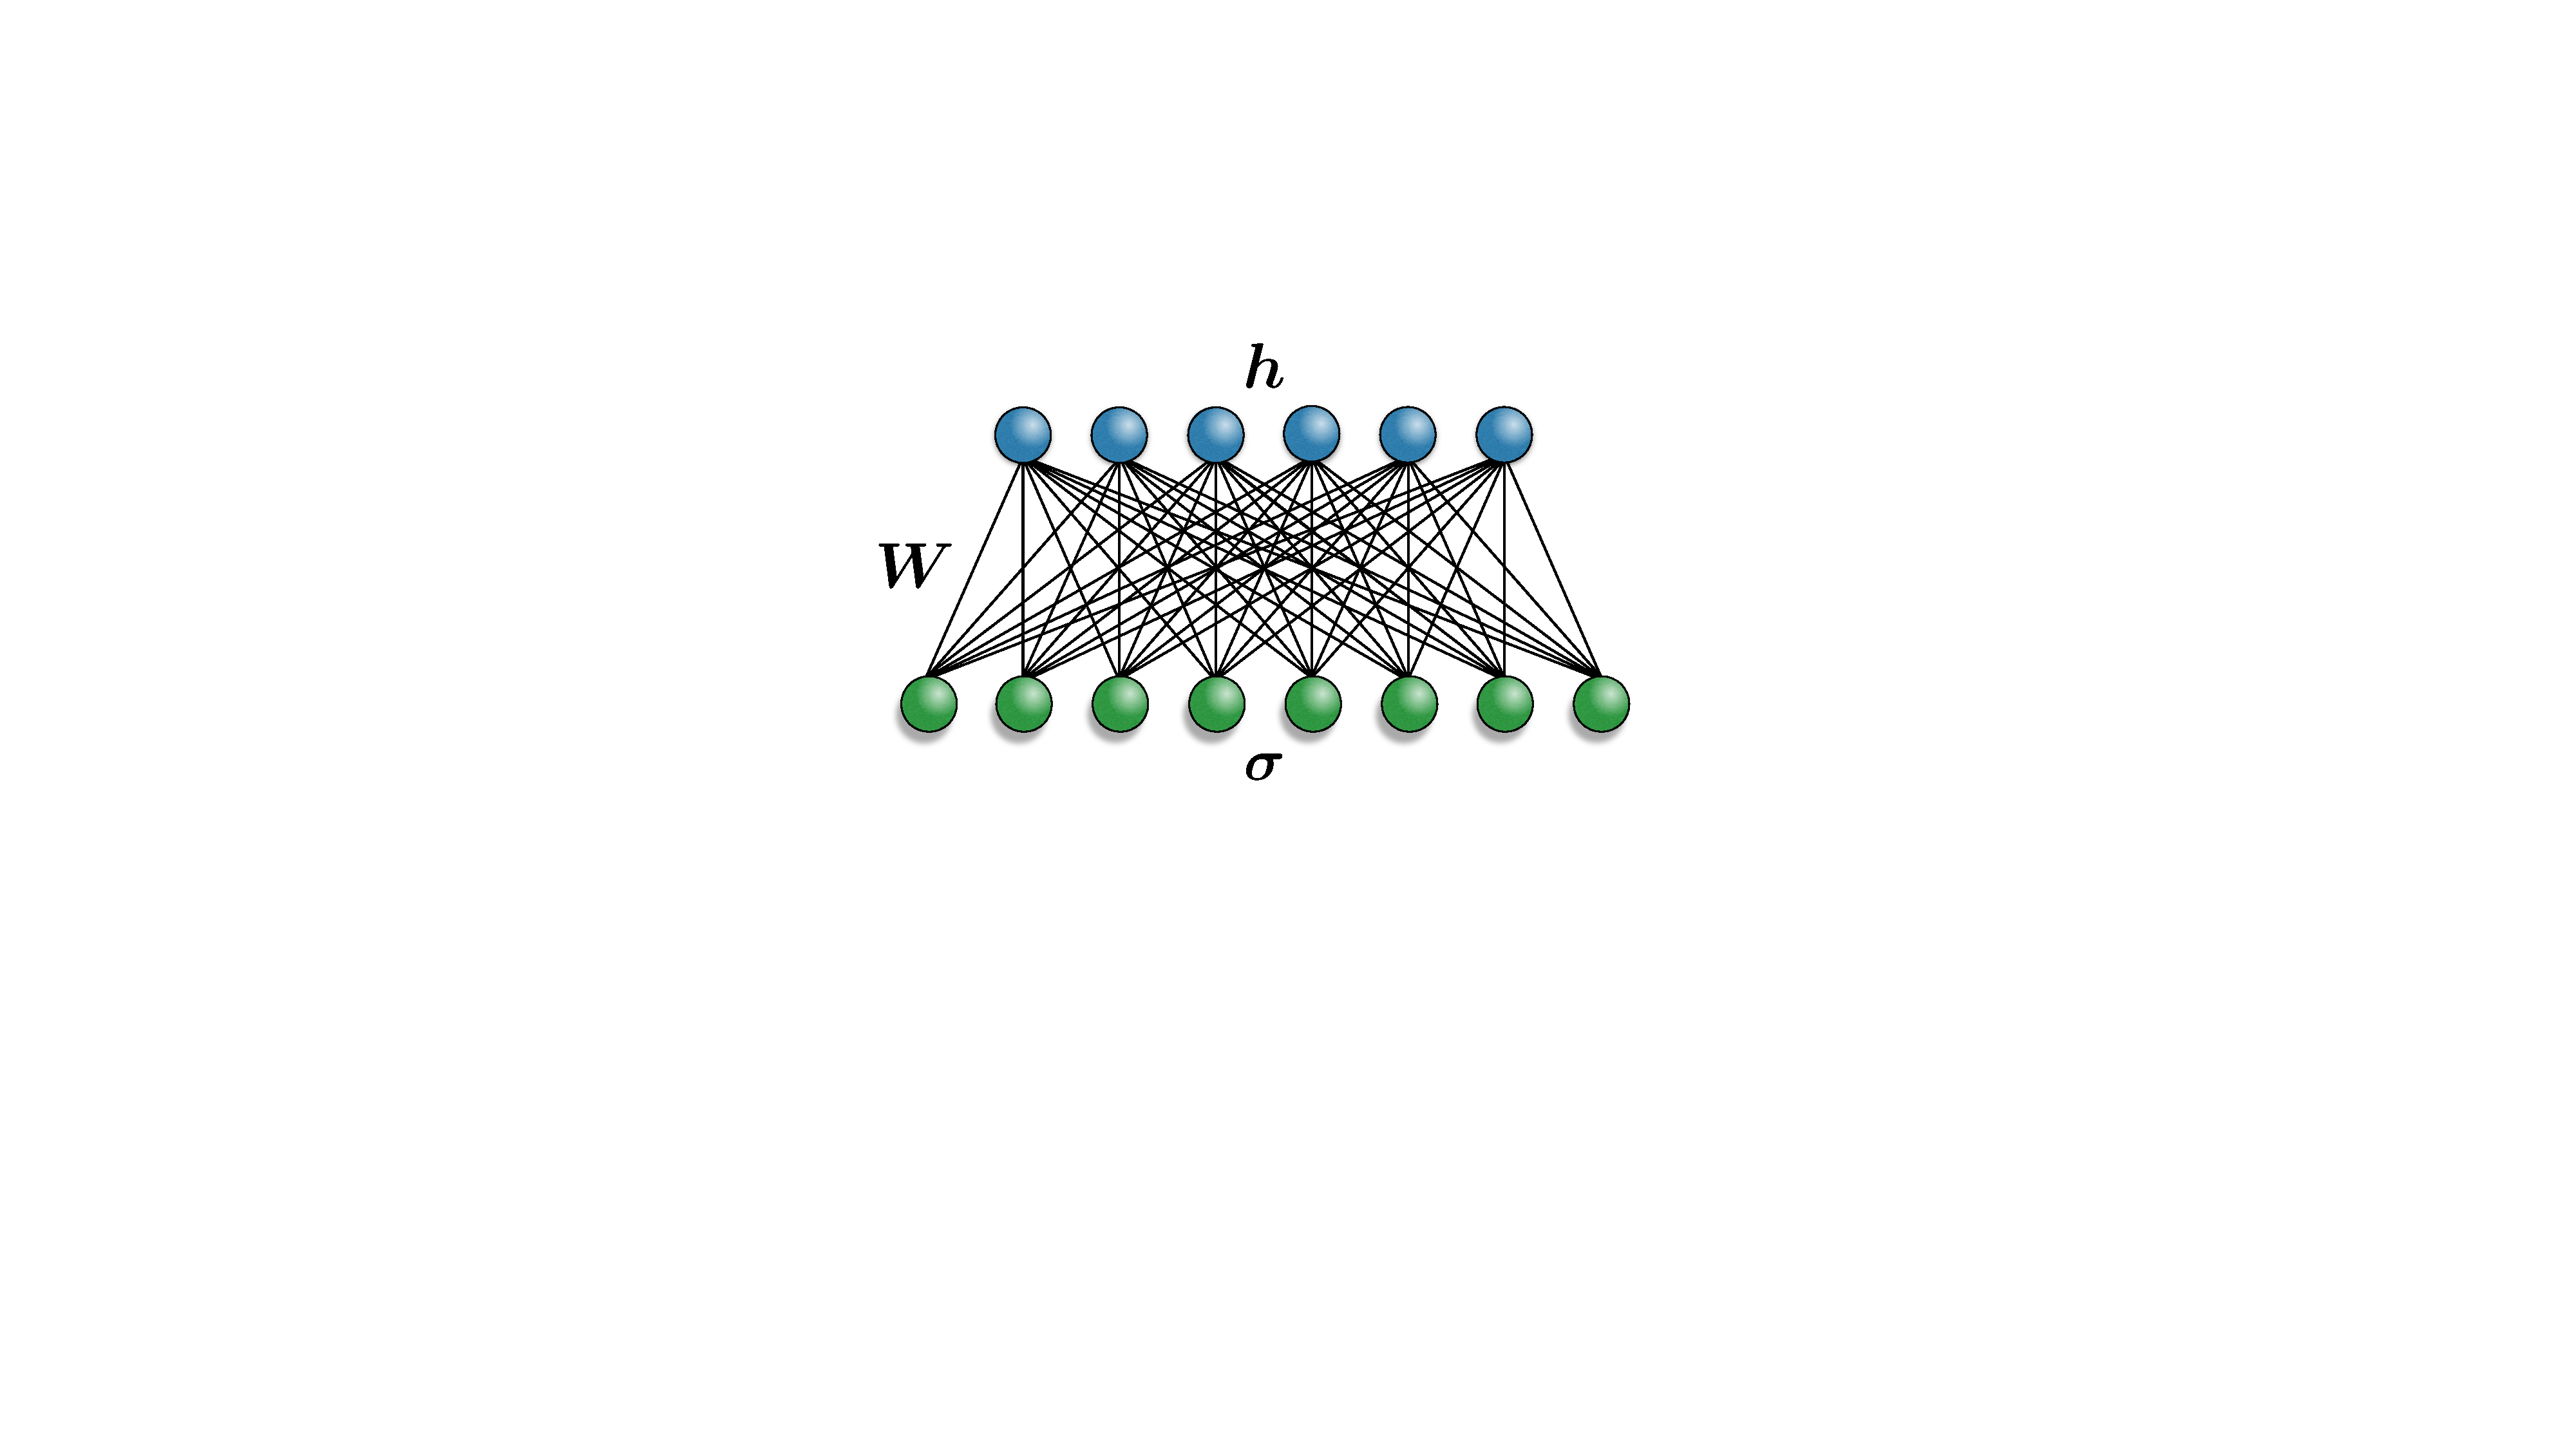
\includegraphics[width=0.5\linewidth]{plots/ch3_positiveNW.pdf}
    \caption{A schematic of the RBM. 
        The visible layer $\bm{\sigma}$ consists of the spins of the quantum system,    
        and the hidden neurons $\bm{h}$ use a sigmoid activation function. 
    The weights, $\bm{W}$, and biases, $\bm{b}$, are optimized through a training procedure.  }
    \label{fig:RBM}
\end{figure}


QuCumber uses contrastive divergence (Appendix~\ref{Glossary}) to determine the most likely state consistent with the given measurements.
As an example, we demonstrate how to train and sample an RBM model with measurements from the one-dimensional transverse-field Ising model.

\subsection{Learning the transverse field Ising model}
\label{Sec:Training_TFIM}

The Hamiltonian for the transverse-field Ising model (TFIM) is
\begin{equation}
	\mathcal{H} = -J\sum_i \sigma^z_i \sigma^z_{i+1} - h \sum_i \sigma^x_i \label{TFIM}	
\end{equation}
where $\sigma^{\alpha}_i$ is a spin-1/2 Pauli operator on site $i$, with $\alpha=x,y,z$. We consider the critical point where $J=h=1$, which is the most difficult state to reconstuct.
For training data, we use a data set consisting of $M=10,000$ measurements in the $\sigma^z$-basis for $N=10$ spins (or qubits), generated with standard numerical techniques~\cite{itensor}.

The example data set is provided in \url{https://github.com/PIQuIL/QuCumber/blob/master/examples/01_Ising/tfim1d_train_samples.txt}.

\subsubsection{An example of measurement data}
\label{subsec:example}

The input data needs to be in a numpy array or a torch tensor.
For a spin system with $N=10$ physical spins and measurements of every spin, one input data point will be an array of the form
\verb|np.array([1,0,1,1,0,1,0,0,0,1])|
, with shape \verb|(N,)|.
Here, we take the representation with $0$ denoting spin-down and $1$, spin-up (in the $\sigma^z$-basis).
All the input data must be an array of these arrays, which will have the shape \verb|(M, N)|, where $M$ is the number of data elements in the training set, and $N$ the number of spins.

We provide a data loading utility to load in the example data set and the exact ground state wavefunction, \verb|true_psi|.
\begin{python}
import qucumber.utils.data as data
psi_path = "tfim1d_psi.txt"
train_path = "tfim1d_data.txt"
train_data, true_psi = data.load_data(train_path, psi_path)
\end{python}

The central object of QuCumber is the representation of the wavefunction, which in the case of a positive-real wavefunction
is a standard RBM as per Figure~\ref{fig:RBM}.
The Python object \verb|PositiveWavefunction| serves this purpose.
To instanciate a positive wavefunction, one needs to specify the number of visible and hidden units in the RBM.
The biases are initialized to zero, and the weights are initalized randomly according to a normal distrubution with zero mean and a variance of $1/$\verb|num_visible|.
\begin{python}
from qucumber.nn_states import PositivWavefunction
state = PositiveWavefunction(num_visible=10, num_hidden=10)
\end{python}
The number of visible units (\verb|num_visible|) is given by the size of the physical system $N$, i.e., the number of spins or qubits.
In contrast, the number of hidden units (\verb|num_hidden|) can be varied to change the expressiveness of the RBM.
Errors in the representation can be systematically improved by increasing the number of hidden units and consequently
the number of parameters (weights and biases) in the network.
Note, the quality of the reconstruction will depend on the specific wavefunction and the ratio $\alpha = \verb|num_hidden|/\verb|num_visible|$.
For some typical examples, we find that $\alpha = 1$ leads to good approximations of positive-real wavefunctions \cite{Torlai2016thermo}.
In the general case, however, the value of $\alpha$ required for a given wavefunction reconstruction should be explored and adjusted by the user.


\subsubsection{Training the RBM}

To train an neural network state, we called the function \verb|PositiveWavefunction.fit|, which takes a number of hyperparameters.
The choice of hyperparameter depends on the details of the system under study, as well as the size and quality of the training set.
In this example, we take a learning rate (\verb|lr|) of $10^{-2}$ using stochastic (batch) gradient descent with a positive (and negative) batch size of 100, trained for 500 epochs.
The number of Gibbs sampling steps \verb|k|, which dictates the number of steps in the contrastive divergence algorithm \cite{hinton2002training},
influences the speed of the training. 


The success of training can be tracked by different measures, like the convergence of the energy or other observables.
In the example of the one-dimensional TFIM, we can compare fidelity of the true ground state with the trained model.
Because of the exponential growth of the wavefunction in the number of qubits, this is only feasible for small physical systems.
Additionally, we calculate the KL-divergence between the distribution of the training data and the distribution of the model.
A correctly trained model should minimize the KL-divergence and maximize the fidelity.

Monitoring training can be done with the use of callbacks, which are are functions that can be evaluated during training.
The first example of a callback is the \verb|MetricEvaluator| which computes any deterministic function every \verb|log_every| epochs during training.
 In this case, we will evaluate the KL divergence and the fidelity with the true ground state included in the training statistics utilities. 
 All necessary arguements to these functions are passed as keyword arguments in \verb|MetricEvaluator|. For the KL divergence, we pass the complete Hilbert space \verb|space|, and for the fidelity we need the exact ground state \verb|true_psi|. 
\begin{python}
from qucumber.callbacks import MetricEvaluator
import qucumber.utils.training_statistics as ts
log_every = 100
space = state.generate_hilbert_space(10)
callbacks = [
    MetricEvaluator(
        log_every,
        {
        "Fidelity": ts.fidelity, 
        "KL": ts.KL, 
        },
    target_psi=true_psi,
    space=space,
    verbose=True
    )
]
\end{python}

Once the metrics to monitor during training have been chosen, we can invoke the optimization with the \verb|fit| function of \verb|PositiveWavefunction|.


\begin{python}
state.fit(
    train_data,
    epochs=400,
    pos_batch_size=100
    neg_batch_size=100,
    lr=0.01
    k=5,
    callbacks=callbacks,
)
\end{python}

With the \verb|verbose=True| option, the program will print the epoch, and all callbacks every \verb|log_every| epochs. These values are plotted in Figure~\ref{fig:KL}. 
The trained RBM and callbacks can saved (or loaded) to a file, and additional data like the fidelity, can we saved as a python dictionary.
\begin{python}
state.save(
    "filename.pt",
    metadata={"fidelity": callbacks[0].Fidelity},
)
state.load("filename.pt")
\end{python}

The metadata can be loaded separately with \verb|torch.load()| which returns a python dictionary.


\begin{figure}[]
    \centering
    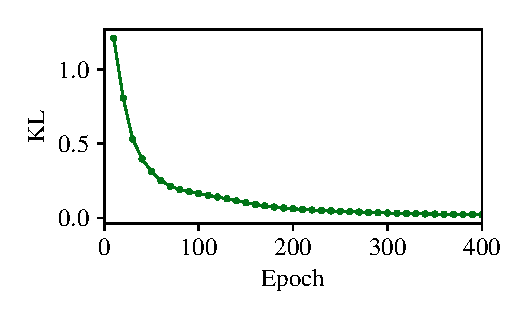
\includegraphics[width=0.48\linewidth, trim={10 14 10 10}, clip]{plots/KL.pdf}
    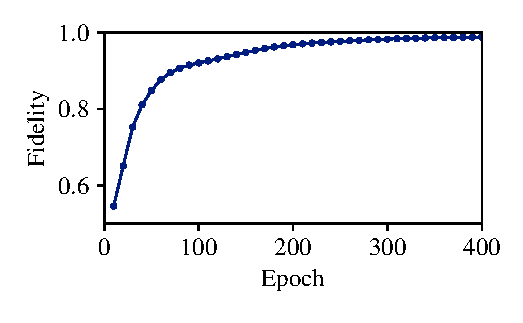
\includegraphics[width=0.48\linewidth, trim={10 14 10 10}, clip]{plots/fid.pdf}
    \caption{The KL divergence (left), and the fidelity (right) during training.
    }
    \label{fig:KL}
\end{figure}

%\section{What can I do with a trained RBM?}

\section{Sampling from a trained RBM}
\label{Sec:Sampling_a-Trained_RBM}

[[ THIS WHOLE SECITON NEEDS SOME LOVE]]

RBMs are generative models, which means that they can produce new configurations of visible and hidden units
drawn according to the learned joint distribution.
These configurations are generated using block Gibbs Sampling and represent a Markov chain. Similar to Monte Carlo techniques, an estimator $\langle \mathcal{O} \rangle$ 
$$
\langle \mathcal{O} \rangle = \frac{1}{\sum_{\bm{\sigma}} |\psi(\bm{\sigma})|^2}
\sum_{\bm{\sigma}}  \mathcal{O}(\bm{\sigma}) |\psi(\bm{\sigma})|^2
$$
can be computed via sampling as 
$$
\langle \mathcal{O}\rangle \approx \frac{1}{N_{\rm MC}} \sum_k^{N_{\rm MC}}  \mathcal{O} (\bm{\sigma'})
$$
with states $ \bm{\sigma'}$ drawn according to the probability distribution from the Born rule.

Some observables only depend on the state under study -- a simple example being the magnetization of any Ising 
system, which can be calculated simply by averaging over all samples $\bm{\sigma}^{(k)}$ in the computational basis.
In QuCumber, one specifies the number of samples and the number of Gibbs steps between samples, $k$:
\begin{python}
samples = state.sample(num_samples=1000, k=10)
\end{python}

The magnetization of these samples can be computer directly. Although somewhat obtuse, the following one-liner converts the binary valued samples to $\pm 1$ spins and computes the average magnetization, $\langle |M|\rangle$,
\begin{python}
magnetization = samples.mul(2.0).sub(1.0).mean(1).abs().mean()
\end{python}

Most observables, however, depend on the Hamiltonian that underlies the original model.
Therefore, we now turn to a discussion of sampling general observables from an RBM.


\subsection{Energy calculation using the Observables module}
[[ESPECIALLY THIS SECITON!] 
%\subsection{Example2: Energy of a TFIM chain}

For the transverse field Ising model a standard observable is the energy, obtained as the expectation value of
the Hamiltonian operator in equation~\ref{TFIM}.
Calculating the energy for a sample $\ket{\bm{\sigma} }= \ket{\sigma_1 \dots \sigma_n}$ is not as straightforward as for the magnetization,
because the Hamiltonian operator ${\sigma}^x_i$ is off-diagonal in the computational basis.

If we write the wavefunction in its expanded form, $\ket{\psi} = \sum_{\bm{\sigma}} \psi(\bm{\sigma}) \ket{\bm{\sigma}} $,
we calculate the expectation value of the Hamiltonian using the local observable,
\begin{align}
    \braket{ \mathcal{H}_L({\bm{\sigma}})} & = \sum_{ \bm{\sigma'}} \mathcal{H}_{\bm{\sigma}, \bm{\sigma}'} \cdot \psi(\bm{\sigma}') / \psi(\bm{\sigma})                                                     \\
	                             & =  \left[ -\sum_i \sigma_i \sigma_{i+1} - h \sum_i \frac{\psi(\sigma_1, \sigma_2, \dots , -\sigma_i, \sigma_{i+1} \dots)}{\psi (\bm{\sigma})} \right]
\end{align}
giving an estimator
\begin{equation}
	\braket{ \mathcal{H}} \approx \frac{1}{M} \sum_k^M \left[ -\sum_i \sigma_i \sigma_{i+1} - h \sum_i \frac{\psi (\bm{\sigma}_{-i})}{\psi (\bm{\sigma})} \right].
\end{equation}
Here we used that $\mathcal{H}_{\bm{\sigma}, \bm{\sigma}'} = \braket{\bm{\sigma} | H | \bm{\sigma}'} = -\sum_i \delta_{\bm{\sigma}, \bm{\sigma}'} - h \sum_i \delta_{\sigma_1, \sigma_1'} \dots \delta_{\sigma_i, -\sigma_i'} \dots$, and defined $\bm{\sigma}_{-i} = \sigma_1, \sigma_2, \dots , -\sigma_i, \sigma_{i+1} \dots$, which is the sample $\bm{\sigma}$ with the $i$-th spin flipped.
% The expectation value can be approximated by drawing $M$ samples and averaging over them.

The sum $\sum_i \sigma_i \sigma_{i+1}$ simply multiplies the neighbouring elements of the sample $\bm{\sigma}$. For the second sum one actually has to calculate the probabilities $\psi (\bm{\sigma})$ of the sample $\bm{\sigma}$ and $\bm{\sigma}_{-i} $ with
$\psi_{\bm{\lambda}}(\bm{\sigma}) = \sqrt{p_{\bm{\lambda}}(\bm{\sigma})}$
%\begin{equation}
%\psi(\bm{\sigma}) = \sqrt{p_{\lambda}(\bm{\sigma})}
%\end{equation}
with $p_{\lambda}(\bm{\sigma})$ (see Eq.~\ref{Eq:marginal_distribution}). The partition functions $Z_{\lambda}$ cancel out if we divide the probabilities and the calculation is tractable also for large system sizes.
The \verb|observable.py| package contains a few examples like this.

[THIS NEEDS TO BE DONE PROPERLY]
\begin{python}
from qucumber.observables import Observable
from quantum_ising_chain import TFIMChainEnergy
TFIM_energy = TFIMChainEnergy(1.0)
energy_stats = tfim_energy.statistics_from_samples(state, samples)
E =energy_stats["mean"]
var = energy_stats["variance"]
\end{python}



\section{Complex wavefunctions}
\label{Sec:Training_QuCumber_on_complex_wavefunctions}

For the positive-real wavefunctions there is no additional information contained in the wavefunction
$\psi( \boldsymbol{\sigma})$ that could be lost by the Born rule that leads to the representation in equation \ref{wfpd}.
However for real wavefunctions for mixed sign, or more generally complex wavefunctions, more care must be taken to ensure 
this phase information is contained in the reconstruction.  

In QuCumber, we represent the phase as an additional RBM with the same visible units but different parameters $\bm{\mu}$. Schematically, the two RBMS are shown in Figure~\ref{fig:complex}
\begin{align}
	\psi_{\bm{\lambda} \bm{\mu}} (\bm{\sigma})= \sqrt{p_{\bm{\lambda}} (\bm{\sigma})} e^{i \phi_{\bm{\mu}} (\bm{\sigma})/2},
\end{align}
%
where we choose $\phi_{\bm{\mu}}(\bm{\sigma}) = \log (p_{\bm{\mu}} (\bm{\sigma}))$ \cite{torlai2018tomography}. 

\begin{figure}[htpb]
    \centering
    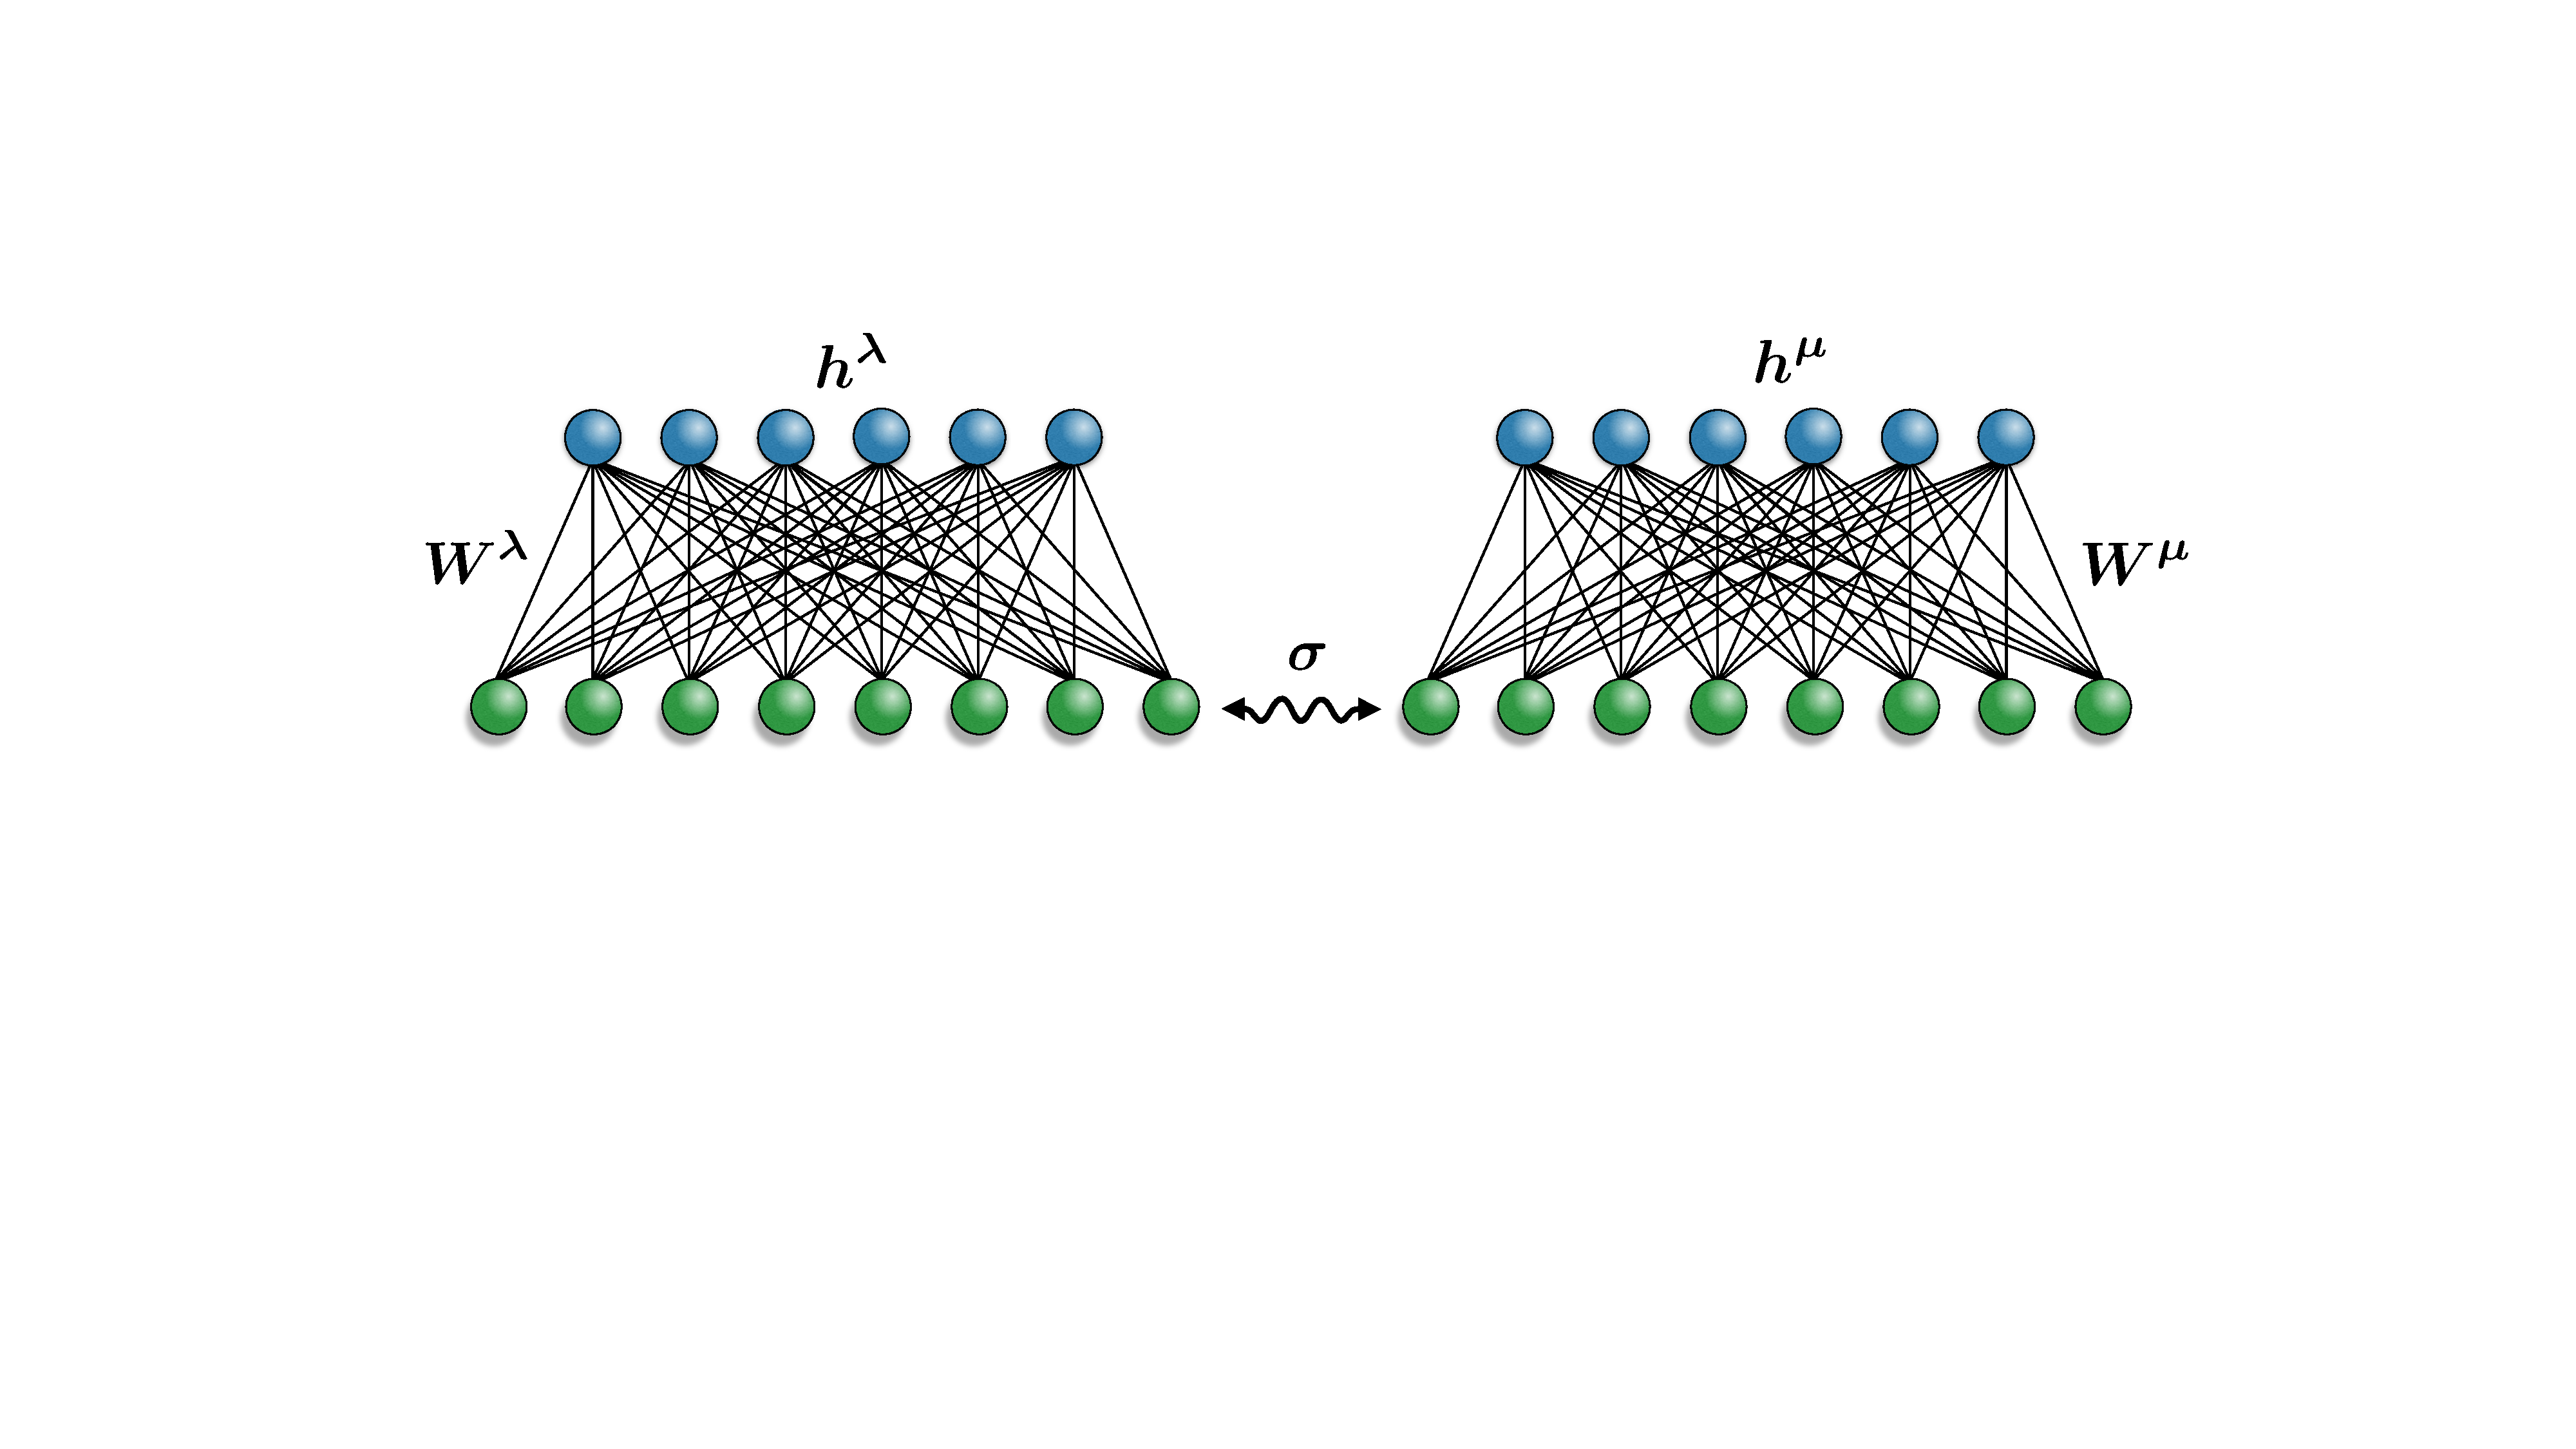
\includegraphics[width=1\linewidth]{plots/ch3_complexNW.pdf}
    \caption{Two RBMs for learning a complex wavefunction. The left RBM with parameters $\bm{\lambda}$ learns the amplitude of the wavefunction, while the parameters $\bm{\mu}$ of the right RBM learn the phase information. Both models input the same visible space, however, the phase information is trained with rotated basis. [EXPLAIN BETTER?]}
    \label{fig:complex}
\end{figure}

The complex wavefunction can be rewritten in a generic basis $\{ \bm{\sigma}^b \}$as :

\begin{align}
	\psi_{\bm{\lambda} \bm{\mu}} (\bm{\sigma}^b)= \sum_{\bm{\sigma}} U (\bm{\sigma}^b, \bm{\sigma}) \psi_{\bm{\lambda} \bm{\mu}} (\bm{\sigma}),
\end{align}
%
with the unitary $U (\bm{\sigma}^b, \bm{\sigma})$ that rotates the state $\ket{\bm{\sigma}^b}$ to $\ket{\bm{\sigma}}$.

---

the phase information contained in these coefficients will be lost if the measurement
is made in only one basis. 
Therefore, in experiments one has to apply local unitary transformations before the measurements
to capture the phase information. Given this additional information one can successfully perform quantum state reconstruction.


Our objective is to learn the full complex wavefunction $\psi_{\bm{\lambda} \bm{\mu}} (\bm{\sigma})$ in the reference basis (in this case, the computational basis) from the measurements of the rotated wavefunction $\psi_{\bm{\lambda} \bm{\mu}} (\bm{\sigma}^b)$.
The RBM again is trained by minimizing the negative log-likelihood (NLL). Following~\cite{} \textbf{ADD REFERENCE TO GIACOMOS THESIS OR SOMETHING THAT SHOWS THE MATH OF THE COMPLEX WAVEFUNCTION}, the gradients of the NLL will contain the unitaries $U (\bm{\sigma}^b, \bm{\sigma})$, and therefore we have to apply a slightly different learning algorithm.

---

In the next two sections, let us consider the example of two qubits, with a general expansion in the computational basis
\begin{equation}
\ket{\psi} = \alpha  \ket{00} + \beta  \ket{01} + \gamma  \ket{10} + \delta \ket{11},
\end{equation}
with arbitrary coefficients $\alpha, \beta, \gamma$ and $\delta$.  We will demonstrate state reconstruction in two ways; first analytically, with a specific chosen set of coefficient; and next numerically using the QuCumber software.

\subsection{An analytical example for two qubits}

It is illustrative to understand the reconstruction technique for complex wavefunctions using an analytical example.  Let us define
the two-qubit state
$\ket{\psi} = 1/2 \{ \ket{00} - \ket{01} + \ket{10} - i \ket{11} \}$.
If we measure the state $\ket{\psi}$ in the computational basis Z, we obtain all qubit states ($\ket{00}$, $\ket{01}$, $\ket{10}$ and $\ket{11}$) with the same probability $p = 1/4$, but we do not learn anything about the phase $i$ or $(-1)$.
Therefore, we apply the local unitaries
\begin{align}
	H = \frac{1}{\sqrt{2}}
	\begin{bmatrix}
		1 & ~1 \\
		1 & -1 \\
	\end{bmatrix},~
	K = \frac{1}{\sqrt{2}}
	\begin{bmatrix}
		1 & -i \\
		1 & ~i \\
	\end{bmatrix}  \label{Unitaries}
\end{align}
on the state before we measure in the computational basis. Measuring the state in the computational basis is equivalent to applying the identity $\mathds{1}$ on the qubits, measuring in the $X$ basis is equivalent to applying a unitary $H$ on the qubit and then measure in $Z$ basis, measuring in $Y$ basis is equivalent to applying a $K$ and then measure in $Z$ basis. Because of the application of local unitaries the probability amplitudes of certain measurement outcomes start mixing and therefore we can extract more information about them. If one applies for example a Hadamard gate $H$ on the second qubit of the state $\ket{\psi}$, we obtain the state:

\begin{align}
	\mathds{1} \otimes H \ket{\psi} & = \frac{1}{2} \{ \ket{0+} - \ket{0-} + \ket{1+} - i \ket{1-} \}          \\
	                                & = \frac{1}{2 \sqrt{2}} \{ 2 \ket{01} + (1-i)\ket{10} + (1+i)\ket{11} \}.
\end{align}

If we measure this state in the Z basis, we obtain the state $\ket{01}$ with probability $p(\ket{01}) = 1/2$
and the other two states with $p(\ket{10}) = p(\ket{11}) = 1/4$.
The state $\ket{00}$ will never be measured. If we repeat the last step with a Hadamard gate on the first qubit, we obtain:
\begin{align}
	H \otimes \mathds{1} \ket{\psi} & = \frac{1}{2} \{ \ket{+0} - \ket{+1} + \ket{-0} - i \ket{-1} \}          \\
	                                & = \frac{1}{2 \sqrt{2}} \{ 2 \ket{00} + (1-i)\ket{01} - (1-i)\ket{11} \}.
\end{align}

Now $p(\ket{00}) = 1/2$, $p(\ket{01}) = p(\ket{11}) = 1/4$ and $p(\ket{10}) = 0$.
We can compare these results to an arbitrary two-qubit state $\ket{\psi}_c = c_1 \ket{00} +c_2 \ket{01} + c_3 \ket{10} +c_4 \ket{11}$,
with all the unitary transformations
\begin{align}
	\mathds{1} \otimes H \ket{\psi}_c & = \frac{1}{2\sqrt{2}} \{ (c_1+c_2) \ket{00} + (c_1 -c_2)\ket{01} + (c_3 + c_4)\ket{10} + (c_3-c_4)\ket{11} \}  \\
	H \otimes \mathds{1} \ket{\psi}_c & = \frac{1}{2\sqrt{2}} \{ (c_1+c_3) \ket{00} + (c_1 -c_3)\ket{01} + (c_2 + c_4)\ket{10} + (c_2-c_4)\ket{11} \}.
\end{align}

From the measurement without unitaries we know that all the probabilities are the same,
which means $c_i \in \{ \pm 1/2, \pm i/2 \}$.
From the application of $H$ to the second qubit we know that $c_1 = -c_2$ and $c_3 = \pm i c_4$.
From the application of $H$ to the first qubit we know that $c_1 = c_3$ and $c_2 = \pm i c_4$.
Already from this information we can do almost full tomography of the state $\ket{\psi}$.
If we fix $c_1 = 1/2$, which just defines a global phase, we find that $c_3 = 1/2$ and $c_2 = -1/2$.
We also find that $c_4 = \pm i/2$.
The only piece that is missing is the sign of $c_4$. To find this sign we apply the unitary $K$ on the second qubit:
\begin{align}
	\mathds{1} \otimes K \ket{\psi} & = \frac{1}{2} \{ \ket{0+} +i \ket{0-} + \ket{1+} - \ket{1-} \}           \\
	                                & = \frac{1}{2 \sqrt{2}} \{ 2 \ket{11} + (1-i)\ket{01} + (1+i)\ket{00} \}.
\end{align}
%
and compare it to the arbitrary state
%
\begin{align}
	\mathds{1} \otimes K \ket{\psi}_c & = \frac{1}{2\sqrt{2}} \{ (c_1-ic_2) \ket{00} + (c_1 +ic_2)\ket{01} + (c_3 -ic_4)\ket{10} + (c_3+ic_4)\ket{11} \},
\end{align}
%
where we find that $c_3 = ic_4$. Therefore, $c_4 = -i$.
Finding the full state $\ket{\psi}$ with this set of unitaries shows that it is a complete set of unitaries.
It might very well be that the complete set also contains the unitary $K \otimes \mathds{1}$,
if the amplitudes of the coefficients were not all the same ($|c_i|^2 \neq 1/4$).

\subsection{A numerical example for two qubits}

In this section we work through a simple numerical example for quantum state reconstruction of a complex two-bit wavefunction with arbitrary coefficients $\alpha, \beta, \delta$ and $\gamma$.  This state is called \verb|target_psi|, described on the online tutorial of the two-qubit example \url{https://github.com/PIQuIL/QuCumber/blob/develop/examples/02_qubits/tutorial_qubits.ipynb}.


First we load the packages needed,

\begin{python}
import torch
import numpy as np
import pickle

from qucumber.nn_states import ComplexWavefunction

from qucumber.callbacks import MetricEvaluator

import qucumber.utils.training_statistics as ts
import qucumber.utils.data as data              
import qucumber.utils.cplx as cplx              
import qucumber.utils.unitaries as unitaries
\end{python}


The data set comprises the measurements \verb|'qubits_train_samples.txt'|, the unitaries that have been applied before the measurement \verb|'qubits_train_bases.txt'| and the actual wavefunction $\ket{\psi}$ the measurements have been sampled from \verb|'qubits_psi.txt'|.

Load the files the following way:

\begin{python}
train_samples_path = 'qubits_train_samples.txt'
train_bases_path   = 'qubits_train_bases.txt'
bases_path         = 'qubits_bases.txt'
psi_path           = 'qubits_psi.txt'

train_samples,target_psi,train_bases,bases = data.load_data(train_samples_path, psi_path, train_bases_path, bases_path)
\end{python}


The training set \verb|train_samples| was measured in the complete basis $\{ZZ, ZX, XZ, ZY, YZ \}$, and therefore \verb|train_bases| contains the unitaries applied to the respective measurement and has the form \verb|np.array([['Z','Z'], ['X','Z'], ['Z','X'], ...])|.
This means that the first measurement has been done in the Z basis for both qubits,
and therefore no unitary has been applied. The second measurement has been done in the XZ basis,
which means that the first qubit has been measured in the X basis. The training of the RBM is analogous to the case of positive-real wavefunction.
We define the training parameters,

\begin{python}
	epochs   = 200
	num_chains = 10
	batch_size = 10
	k     = 10
	lr     = 0.1
	log_every = 10
\end{python}

initialize the wavefunctions:

\begin{python}
nn_state.space = nn_state.generate_hilbert_space(nv) # generate the entire visible space of the system.
callbacks      = [MetricEvaluator(log_every,{'Fidelity':ts.fidelity,'KL':ts.KL},target_psi=target_psi,bases=bases,
                                  verbose=True, space=nn_state.space)]
# The "verbose=True" argument will print the parameters in { } as a function of the training process.
\end{python}

and start the training:

\begin{python}
nn_state.fit(train_samples, epochs, batch_size, num_chains, CD,
       lr, input_bases=train_bases, progbar=False, callbacks=callbacks)
\end{python}

After the training we can calculate state fidelity, observables or sample from the complex wavefunction
the same way we did from the real-positive wavefunction. However, one has to keep in mind that the sampling only works in the Z basis.

\subsection{Defining general unitaries}

QuCumber contains by default the unitaries $\mathds{1}$, $H$ and $K$ (see equation \ref{Unitaries}).
%\begin{align}
%	\mathds{1} =
%	\begin{bmatrix}
%		1 & 0 \\
%		0 & 1 \\
%	\end{bmatrix},~
%	H = \frac{1}{\sqrt{2}}
%	\begin{bmatrix}
%		1 & ~1 \\
%		1 & -1 \\
%	\end{bmatrix},~
%	K = \frac{1}{\sqrt{2}}
%	\begin{bmatrix}
%		1 & -i \\
%		1 & ~i \\
%	\end{bmatrix}
%\end{align}
Additional new basis transformations can be added in the following way:
\begin{python}
	from qucumber import unitary
	import numpy as np
	new_unitary
	unitary_dict = unitaries.create_dict(name = 'new_unitary', unitary = new_unitary)
\end{python}
This creates a new unitary instance which is called \verb|'new_unitary'| and connects this name with the \verb|numpy| array
\verb|new_unitary| that has the form \verb|A = np.array([a,b],[c,d]])| for a matrix

\begin{align}
	A =
	\begin{bmatrix}
		a & b \\
		c & d \\
	\end{bmatrix}.
\end{align}

To call this basis transformation during the training, an element of the \verb|train_bases| array from above has to have the form
\verb|np.array(['Z','new_unitary'])| for a two-qubit example,
which means before the measurement the \verb|new_unitary| was applied to the second qubit.

So far we only used maximally one local unitary that is not the identity, such that maximally one qubit was not measured in the \verb|'Z'| basis.
QuCumber provides also the possibility for an arbitrary number \textcolor{red}{It is not really arbitrary, is there a maximum implemented} of non-trivial unitaries per measurement.
An element of \verb|train_bases|, for example, for a six-qubit state could have the following form:
\verb|np.array(['X','Z','new_unitary','Z','Y','X'])|

Apart from the training there is no difference in the positiv-real and the complex wavefunctions. The observables and callbacks are caculated as described in Section \ref{Sec:Sampling_a-Trained_RBM} and \ref{Sec:Callbacks}.
The sampling from the RBM is also exactly the same for both cases.
In the complex case, sampling from the RBM can only be performed in the original basis, which in our case was the Z basis.
\textcolor{red}{[what's correct? Double check this with code]}
%\section{Off diagonal observables in a trained complex wavefunction}
%
%We might add here an example for a non-trivial observable for complex wavefunctions.

\section{Conclusion}

We introduced the open-source package QuCumber for quantum state tomography with Restricted Boltzmann Machines and demonstrated on examples that
the package is applicable on positive-real and complex wavefunctions for any possible physical system with binary measurement outputs.
The class provided for the case of positive-real wavefunctions is highly parallelizable on GPUs and exhibits very high performance.
For complex wavefunctions QuCumber provides standard local unitaries for basis transformations
and can easily be equipped with customized unitaries, and therefore applied on any system with binary measurement outcomes.
After successful training of the RBM, one has full access to the wavefunction, respectively to the probability distribution of the measurements of the system.
One can sample new measurements, calculate observables or the fidelity to any other state.
We provide example code for any of these tasks to give the user a first impression of the implementation of

In the future QuCumber will be extended to the application of quantum state tomography on mixed states, multinomial quantum systems (like boson systems) and eventually on continuous variable systems.

\section*{Acknowledgements}
We acknowledge G. Carleo, J. Carrasquilla and L. Hayward Sierens for stimulating discussions.  
We thank J. Matlock and the Perimeter Institute for Theoretical Physics for the continuing support of PIQuIL.

% TODO: include author contributions
\paragraph{Author contributions}
Authors are listed alphabetically. For an updated record of individual contributions, consult the repository at \url{https://github.com/PIQuIL/QuCumber/graphs/contributors}.

% TODO: include funding information
\paragraph{Funding information}
P.H. acknowledges support from ICFOstepstone - PhD Programme for Early-Stage Researchers in Photonics, funded by the Marie Sklodowska-Curie Co-funding of regional, national and international programmes (GA665884) of the European Commission, as well as by the Severo Ochoa 2016-2019' program at ICFO (SEV-2015-0522), funded by the Spanish Ministry of Economy, Industry, and Competitiveness (MINECO).
R.G.M. is supported in part by funding from the Natural Sciences and Engineering Research Council of Canada (NSERC) and a Canada Research Chair.
Research at Perimeter Institute is supported by the Government of Canada through Industry Canada and by the Province of Ontario through the Ministry of Research \& Innovation.


\appendix
\section{Glossary}
\label{Glossary}

We list an overview of terms discussed in the document and relevant for RBMs. For more detail we refer to the code documentation on \url{https://piquil.github.io/QuCumber/}, and References~\cite{hinton2002training, hinton2012practical}.

\begin{itemize}

	\item {\it Batch}: The subset of data selected for one iteration of training in stochastic gradient descent.

	\item {\it Biases}: For a visible unit $v_j$ and a hidden unit $h_i$, the respective biases in the RBM energy are $b_j$ and $c_i$. They act like a magnetic field term in the energy Eq~(\ref{RBMenergy}).

	\item {\it Contrastive Divergence}: An approximate maximum-likelihood learning algorithm for RBMs \cite{hinton2002training}.

	\item {\it Energy}: In analogy to statistical physics the energy of an RBM is defined given the joint configuration $(v,h)$ of visible and hidden units:
	      \begin{equation}
		      E_{\bm{\lambda}}(v,h) = - \sum\limits_{j=1}^V b_j v_j - \sum\limits_{i=1}^H c_i h_i - \sum\limits_{ij} h_i W_{ij} v_j, \label{RBMenergy}
	      \end{equation}

	\item {\it Effective energy}: Energy traced over the hidden units $h$.  Often called the ``free energy'' in machine learning literature.
	      \begin{equation}
		      \mathcal{E}_{\bm{\lambda}}(v) = - \sum\limits_{j=1}^V b_j v_j - \sum\limits_{i=1}^H \log \left\{ 1 + \exp \left( \sum\limits_{j} W_{ij}v_j +c_i\right) \right\}, \label{RBMeffectiveenergy}
	      \end{equation}

	\item {\it Epoch}: A single pass through an entire training set of data.

	\item {\it Hidden Units}: There are $H$ units in the second layer of the RBM, denoted by the vector $h=(h_1, ..., h_H)$, representing latent variables and are referred to as ``hidden". The number of hidden units $H$ can be adjusted to tune the representational capacity of the RBM.

	\item{\it Hyperparameter:} RBM architecture, and some details of training, that are fixed before training begins.  Examples are the learning rate, number of hidden units, batch size, or number of training epochs.

	\item {\it Joint distribution}: The RBM assigns a probability to each joint configuration $(v,h)$ according to the Boltzmann distribution of the energy,
	      \begin{equation}
		      p_{\bm{\lambda}}(v,h) = \frac{1}{Z_{\bm{\lambda}}} e^{-E_{\bm{\lambda}}(v,h)},
	      \end{equation}
	      
	      \item{\it KL-divergence}: The Kullback-Leibler divergence, or relative entropy, is a measure the distance between two probability distributions.

\item{\it Learning Rate}: A hyperparamter that can be adjusted to affect training performance.  Training speed is proportional to the learning rate, however the chance of finding a good minimum to the KL-divergence is higher for low learning rates.


	\item {\it Marginal distribution}: Obtained by marginalizing the joint distribution, e.g.
	      \begin{equation}
		      \label{Eq:marginal_distribution}
		      p_{\bm{\lambda}}(v) = \frac{1}{Z_{\bm{\lambda}}} \sum\limits_{h\in \mathcal{H}} e^{-E_{\bm{\lambda}}(v,h)} = \frac{1}{Z_{\bm{\lambda}}} e^{- \mathcal{E}_{\bm{\lambda}}(v)}.
	      \end{equation}

	\item {\it QuCumber}: A quantum calculator used for many-body eigenstate reconstruction.

	\item {\it Parameters}: An RBM's energy is defined via a set of neural network parameters $\bm{\lambda} = \{b,c,W\}$, consisting of weights and biases.

	\item {\it Partition function}: The normalizing constant of the Boltzmann distribution. It is obtained by summing over all possible pairs of visible and hidden vectors,
	      \begin{equation}
		      Z_{\bm{\lambda}} = \sum\limits_{v\in \mathcal{V}}\sum\limits_{h\in \mathcal{H}} e^{-E_{\bm{\lambda}}(v,h)}.
	      \end{equation}

	\item {\it Restricted Boltzmann Machine}: A two-layer network with bidirectionally connected stochastic processing units. ``Restricted" refers to the connections (or weights) between the visible and hidden units. Each visible unit is connected with each hidden unit, but there are no intra-layer connections.

	\item {\it Visible Units}: There are $V$ units in the first layer of the RBM, denoted by the vector $v=(v_1, ..., v_V)$, which correspond to the experimental data and are therefore called ``visible". The number of visible units $V$ is fixed to the number of physical qubits.

	\item {\it Weights}: $W_{ij}$ is the symmetric connection or interaction between the visible unit $v_j$ and the hidden unit $h_i$.

\end{itemize}



	\section{Algorithm for a real positive wavefunction}
	The training algorithm of the RBM has the following structure.
	%=================================================================================
	% RBM.train

	\begin{algorithm}[H]
		\caption{Training Algorithm of QuantumReconstruction. \textbf{QR.train}() }
		\SetAlgoLined
		\For{batch in training set}{
			Load batch from training set, batch $=(\hat{ \boldsymbol{\sigma}}_1~\hat{ \boldsymbol{ \sigma}}_2 \dots)$\;
			compute the gradients from the batch $\Delta \bm{\Theta } =$ ($\Delta W$, $\Delta b$, $\Delta c$)\\
			\textbf{\lstinline{QR.compute_batch_gradients}}(k, batch, basis)  \Comment*[r]{Algorithm 2}
			update weights and biases \\
			$\bm{\Theta} \leftarrow \bm{\Theta } - \Delta \bm{\Theta } $ \;
		}

	\end{algorithm}

	%=================================================================================
	% RBM.compute gradient

	The gradients are calculated according to the contrastive divergence algorithm, which allows us to approximate the probability distribution of the model with $k$ Gibbs sampling steps from the actual training data.

	\begin{algorithm}[H]
		\caption{Compute Gradient from Batch. \textbf{\lstinline{QR.compute_batch_gradients}}(k, batch, basis) }
		\SetAlgoLined
		\uIf{basis = None}{
			Reset gradients $\Delta W$, $\Delta h_b$, $\Delta v_b$ $= 0$\;
			\For{$\hat{ \boldsymbol{ \sigma}}_i$ in batch}{
				sample $\bm{h}_0$, $\bm{v}_k$ and $\bm{p}_{h_k}$ from $\hat{ \boldsymbol{ \sigma}}_i$\\
				\textbf{\lstinline{RBM.gibbs_sampling}}(k, $\hat{ \boldsymbol{ \sigma}}_i$)  \Comment*[r]{Algorithm 3}
					calculate gradients\\
				$\Delta W += \bm{v}_0 \bm{h}_0^T - \bm{v}_k \bm{p}_{h_k}^T$ \\
				$\Delta c += \bm{h}_0 - \bm{p}_{h_k}$ \\
				$\Delta b += \bm{v}_0 - \bm{v}_k$ \;
			}
			$M = \vert batch \vert$ \;
			return $\Delta W / M$, $\Delta c / M$, $\Delta b / M$ \;}
		\Else{Do complex gradient \Comment*[r]{Algorithm 6}}
	\end{algorithm}

	%=================================================================================
	% RBM.gibbs sampling

	The Gibbs sampling is done $k$ times back and forth. The contrastive divergence algorithm already shows good results for $k=1$. But for better results this value can be increased.

	\begin{algorithm}[H]
		\caption{Gibbs sampling. \textbf{\lstinline{RBM.gibbs_sampling}}(k, $\hat{ \boldsymbol{ \sigma}}_i$) }
		\SetAlgoLined
		calculate $\bm{p}_h$ and sample $\bm{h}_0$ from $\hat{ \boldsymbol{ \sigma}}_i$\\
		\textbf{\lstinline{RBM.sample_h_given_v}}($\hat{ \boldsymbol{ \sigma}}$)  \Comment*[r]{Algorithm 4}
		$\bm{h} = \bm{h}_0$\;
			i = 0\;
			\While{i $\leq$ k}{
				calculate $\bm{p}(\bm{v}|\bm{h}_i)$ and sample $\bm{v}$ from $\bm{h}$\\
				\textbf{\lstinline{RBM.sample_v_given_h}}($\bm{h}$)  \Comment*[r]{Algorithm 5}
					calculate $\bm{p}(\bm{h}|\bm{v})$ and sample $\bm{h}$ from $\bm{v}$\\
					\textbf{\lstinline{RBM.sample_h_given_v}}($\bm{v}$)  \Comment*[r]{Algorithm 4}
				$i +=1$
			}
			return $\bm{p}_{h_k} =$ $\bm{p}(\bm{h}|\bm{v})$, $\bm{v}_k = \bm{v}$ and $\bm{h}_0$\;

	\end{algorithm}


	%=================================================================================
	% RBM.v given h and vice versa



	\begin{algorithm}[H]
		\caption{calculate $\bm{p}(\bm{v}|\bm{h})$ and sample $\bm{v}$ \textbf{\lstinline{RBM.v_given_h}}() }
		\SetAlgoLined
		calculate probability $\bm{p}(\bm{v} = 1|\bm{h}) = \sigma( W \bm{h} + v_b)$\;
		Bernoulli sample $\bm{v}$ from this probability\;
		return $\bm{v}$ and $\bm{p}(\bm{v} = 1|\bm{h})$\;

	\end{algorithm}


	\begin{algorithm}[H]
		\caption{calculate $\bm{p}(\bm{h}|\bm{v})$ and sample $\bm{h}$ \textbf{\lstinline{RBM.h_given_v}}() }
		\SetAlgoLined
		calculate probability $\bm{p}(\bm{h} = 1|\bm{v}) = \sigma(\bm{v}^T W + h_b)$\;
		Bernoulli sample $\bm{h}$ from this probability\;
		return $\bm{h}$ and $\bm{p}(\bm{h} = 1|\bm{v})$\;

	\end{algorithm}

% TODO:
% Provide your bibliography here. You have two options:

% FIRST OPTION - write your entries here directly, following the example below, including Author(s), Title, Journal Ref. with year in parentheses at the end, followed by the DOI number.
%\begin{thebibliography}{99}
%\bibitem{1931_Bethe_ZP_71} H. A. Bethe, {\it Zur Theorie der Metalle. i. Eigenwerte und Eigenfunktionen der linearen Atomkette}, Zeit. f{\"u}r Phys. {\bf 71}, 205 (1931), \doi{10.1007\%2FBF01341708}.
%\bibitem{arXiv:1108.2700} P. Ginsparg, {\it It was twenty years ago today... }, \url{http://arxiv.org/abs/1108.2700}.
%\end{thebibliography}

% SECOND OPTION:
% Use your bibtex library
% \bibliographystyle{SciPost_bibstyle} % Include this style file here only if you are not using our template
\bibliography{bibliography}

\nolinenumbers

\end{document}
